\begin{frame}[parent={cmap:coverage-analysis-tool},hasnext=true,hasprev=true]
\frametitle{Coverage analysis tool}
\framesubtitle{Visualization of definition-use graph}
\label{concept:jabuti-visualization}

\begin{block:fact}{Visualization}
\begin{itemize}
	\item JaBUTi generates, for every method, a definition-use graph,
	 as well as the visualization of the bytecode and of the source code
	 (when available).
\end{itemize}
\end{block:fact}

\begin{block:fact}{Available information}
\begin{itemize}
	\item For each node in the graph, the following information is available:
	\begin{itemize}
		\item set of variables used,
		\item set of variables defined,
		\item corresponding source code lines,
		\item corresponding bytecode ``line'' (PC).
	\end{itemize}
\end{itemize}
\end{block:fact}
\end{frame}


\begin{frame}
\frametitle{Coverage analysis tool}
\framesubtitle{Visualization of definition-use graph}

\begin{block:fact}{Source code and bytecode}
\begin{itemize}
	\item The corresponding source code of the current class is displayed in
	colors, mapped back from the bytecode, facilitating the
	identification of which part of the source code should be covered first.
\end{itemize}
\end{block:fact}

\begin{center}
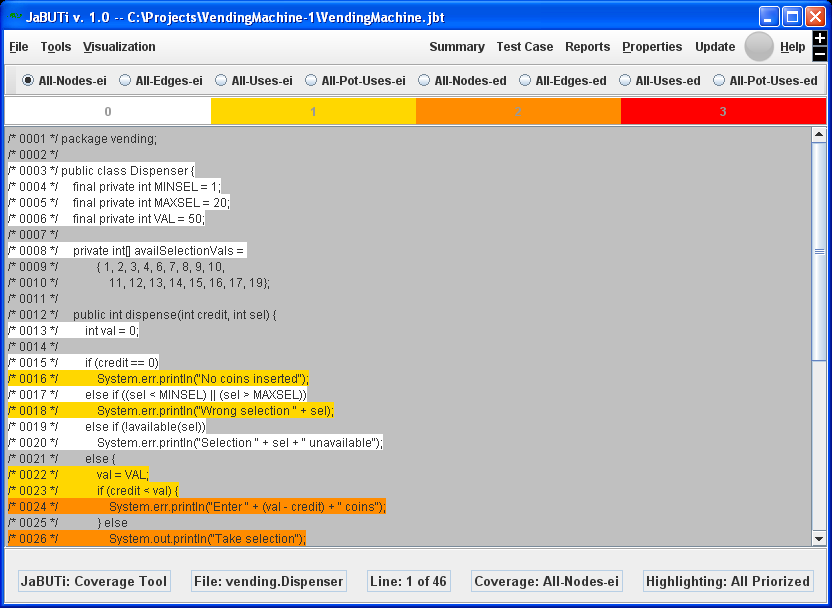
\includegraphics[width=.5\textwidth]{resources/JaBUTi/JaBUTi-VendingMachine/JaBUTi-VendingMachine-Visualization-SourceCode}
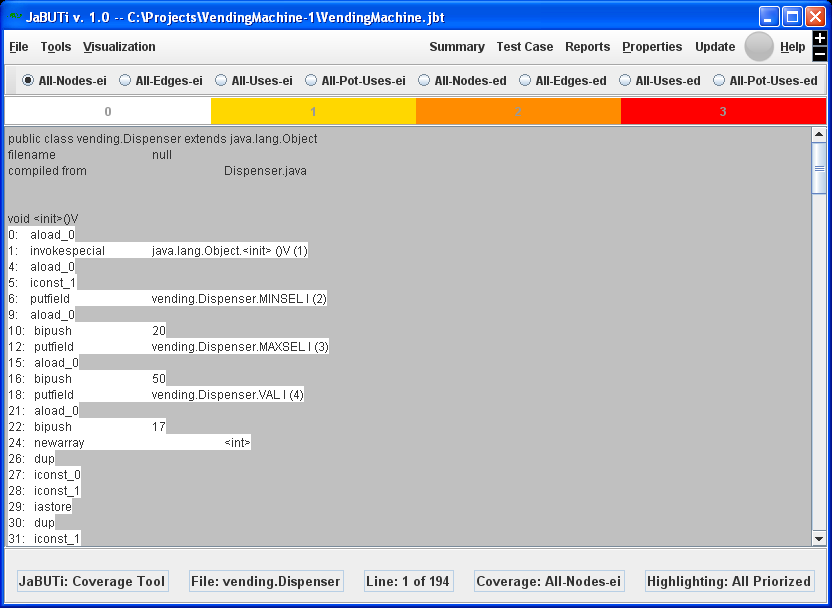
\includegraphics[width=.5\textwidth]{resources/JaBUTi/JaBUTi-VendingMachine/JaBUTi-VendingMachine-Visualization-Bytecode}
\end{center}
\end{frame}


\begin{frame}
\frametitle{Coverage analysis tool}
\framesubtitle{Visualization of definition-use graph}

\begin{block:fact}{DUG representation}
\begin{itemize}
	\item JaBUTi represents the definition-use graph using three different
	types of nodes -- common nodes, exit nodes, and call nodes -- and two
	different types of edges -- primary edges, and secundary edges.

	\item JaBUTi represents:
	\begin{itemize}
		\item common nodes with single-lined circles,

		\item exit nodes with bold single-lined circles,

		\item call nodes with double-lined circles,

		\item primary edges with continuous lines,

		\item secondary edges with dashed lines.
	\end{itemize}
\end{itemize}
\end{block:fact}
\end{frame}



\begin{frame}[c]
\frametitle{Coverage analysis tool}
\framesubtitle{Visualization of definition-use graph}

\begin{center}
\animategraphics[height=160pt,poster=first,autoplay,loop]{1}{main/coverage-analysis-tool/jabuti-visualization-dug-}{0}{1}
\end{center}
\end{frame}


\begin{frame}
\frametitle{Coverage analysis tool}
\framesubtitle{Visualization of definition-use graph}

\begin{block:fact}{Test requirement weight}
\begin{itemize}
	\item Depending on which test criterion is active, the bytecode, source
	code and definition-use graph is colored in a different way in JaBUTi.

	\item The colors represents the weight of the test requirements.
	\begin{itemize}
		\item A test requirement with weight zero (a covered requirement) is
		painted in white.
	\end{itemize}
\end{itemize}
\end{block:fact}
\end{frame}



\begin{frame}
\frametitle{Coverage analysis tool}
\framesubtitle{Visualization of definition-use graph}

\begin{block}{Example}
\insertmovie{resources/JaBUTi/JaBUTi-VendingMachine/JaBUTi-VendingMachine-Visualization/JaBUTi-VendingMachine-Visualization}
\end{block}
\end{frame}
